\documentclass{standalone}
\usepackage{pgfplots}
\pgfplotsset{compat=newest}

\begin{document}
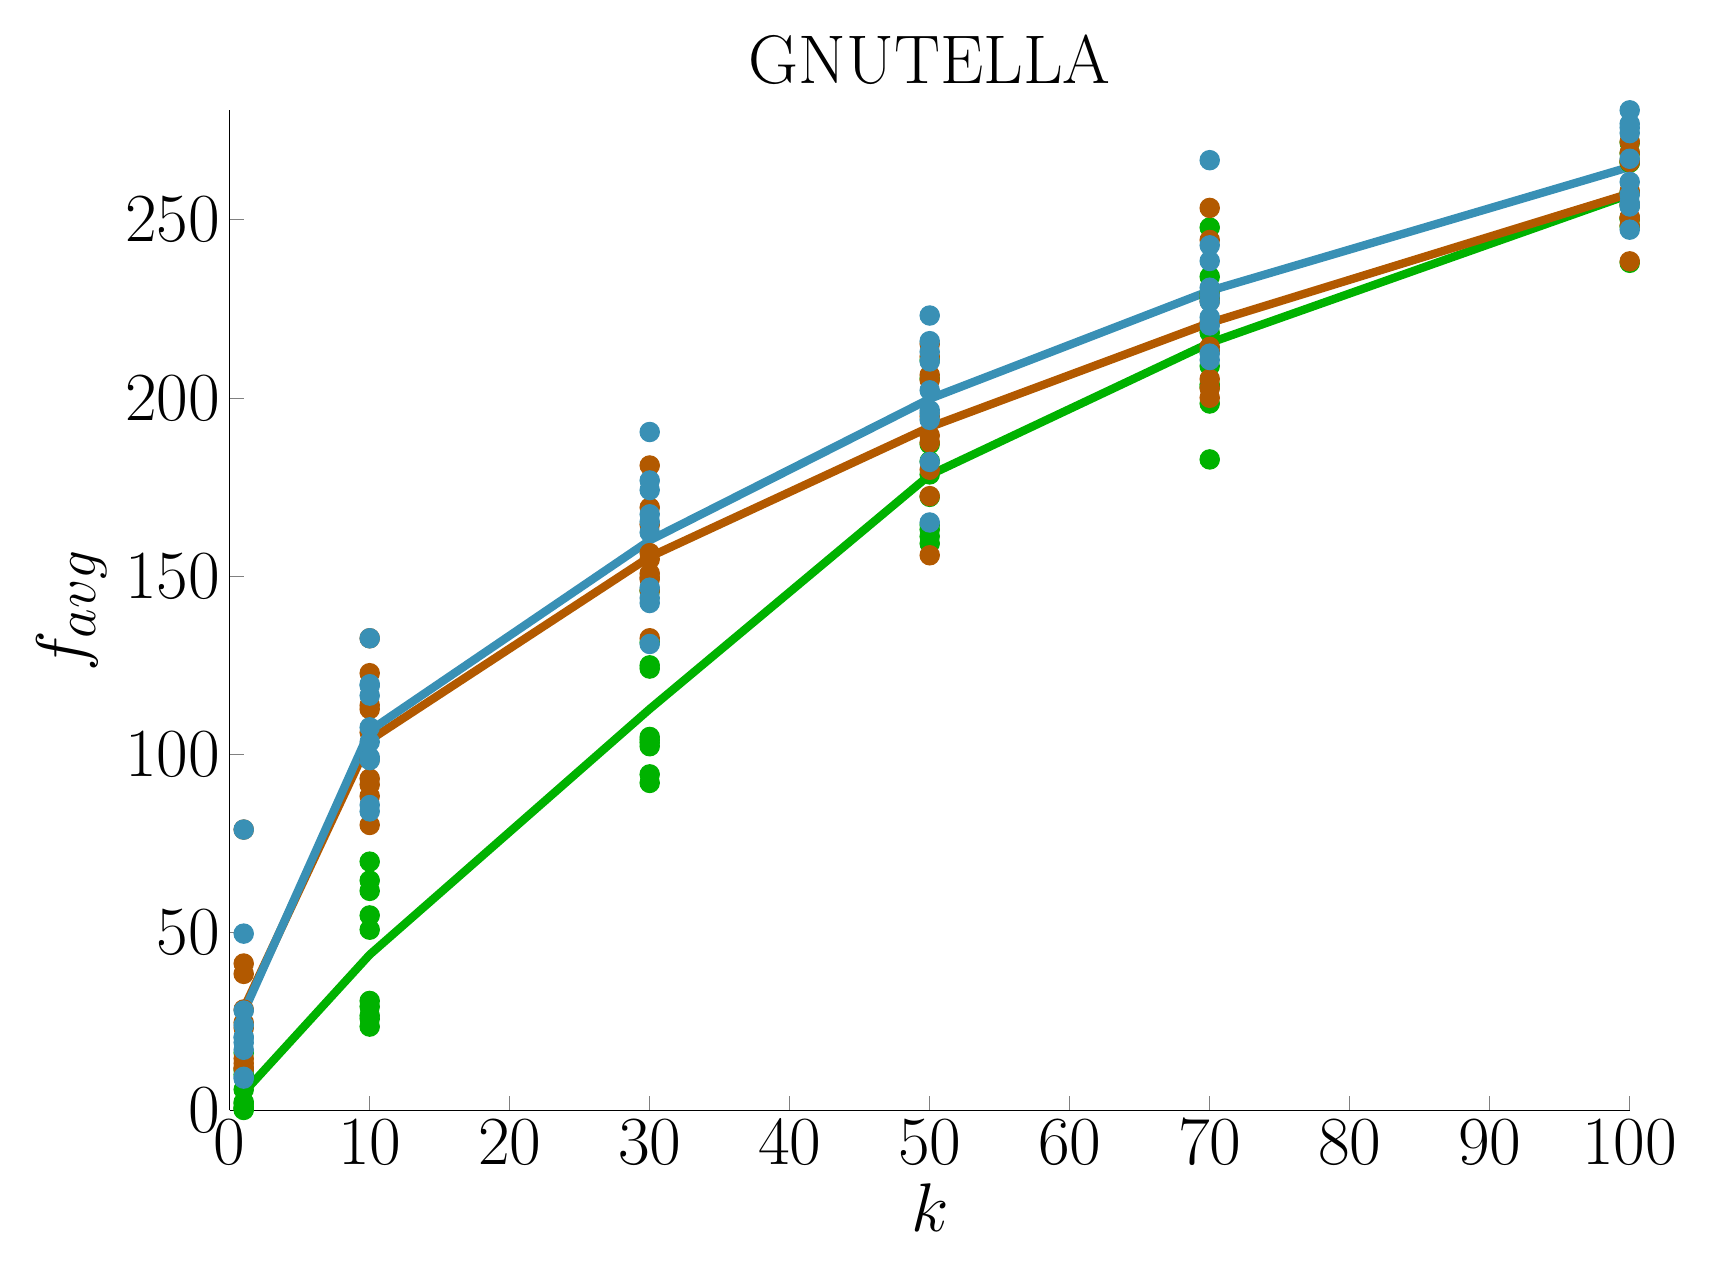
\begin{tikzpicture}

\begin{axis}[%
title style={font=\Huge},
title=GNUTELLA,
tick label style={font=\Huge},
label style={font=\Huge},
legend style={font=\Huge},
view={0}{90},
max space between ticks=50pt,
width=7in,
height=5in,
scale only axis,
xmin=0, xmax=100,
%xtick={0, 20, 40, 60, 80, 100},
xlabel={$k$},
ymin=0, ymax=280.7,
ylabel={$f_{avg}$},
major tick length=5pt,
axis lines*=left,
legend cell align=left,
clip=false]

\addplot [
only marks,
mark=*,
mark size=3.5pt,
color=green!70!black,
%solid,
%line width=2pt,
]
coordinates{
(1,0.1)(1,0.5)(1,0.6)(1,0.9)(1,1.9)(1,2.3)(1,5.8)(1,10.1)(1,11.3)(1,16.1)(10,23.5)(10,25.7)(10,26.6)(10,29.1)(10,30.7)(10,50.7)(10,54.7)(10,61.6)(10,64.5)(10,69.8)(30,91.9)(30,94.3)(30,102.2)(30,103.2)(30,104.0)(30,104.8)(30,124.0)(30,124.9)(30,131.4)(30,145.8)(50,159.1)(50,161.1)(50,163.0)(50,164.3)(50,172.2)(50,178.5)(50,182.2)(50,187.0)(50,205.4)(50,210.6)(70,182.7)(70,198.4)(70,203.0)(70,203.7)(70,208.9)(70,218.3)(70,228.0)(70,229.2)(70,234.0)(70,247.8)(100,237.9)(100,248.1)(100,250.1)(100,250.4)(100,254.1)(100,257.6)(100,266.0)(100,266.2)(100,268.6)(100,271.6)
};

\addplot [
only marks,
mark=*,
mark size=3.5pt,
color=orange!70!black,
%solid,
%line width=2pt,
]
coordinates{
(1,11.7)(1,11.9)(1,13.2)(1,14.5)(1,23.1)(1,24.6)(1,28.3)(1,38.3)(1,41.2)(1,78.8)(10,80.1)(10,88.2)(10,91.4)(10,93.1)(10,98.5)(10,106.1)(10,112.6)(10,113.7)(10,122.7)(10,132.5)(30,132.5)(30,145.9)(30,149.1)(30,149.6)(30,150.7)(30,154.7)(30,156.4)(30,164.4)(30,169.2)(30,181.0)(50,155.8)(50,172.4)(50,179.8)(50,187.5)(50,189.4)(50,194.8)(50,205.0)(50,206.4)(50,211.6)(50,215.1)(70,200.0)(70,202.7)(70,205.3)(70,213.2)(70,214.3)(70,221.3)(70,227.1)(70,228.8)(70,244.3)(70,253.3)(100,238.3)(100,248.4)(100,250.6)(100,250.6)(100,254.1)(100,258.0)(100,266.2)(100,266.6)(100,268.8)(100,271.9)
};

\addplot [
only marks,
mark=*,
mark size=3.5pt,
color=cyan!70!black,
%solid,
%line width=2pt,
]
coordinates{
(1,8.9)(1,9.4)(1,17.0)(1,19.0)(1,20.5)(1,20.5)(1,23.9)(1,28.0)(1,49.6)(1,78.8)(10,83.9)(10,85.7)(10,98.3)(10,99.1)(10,103.4)(10,107.5)(10,116.4)(10,119.2)(10,119.6)(10,132.5)(30,130.9)(30,142.4)(30,143.8)(30,146.7)(30,162.2)(30,165.2)(30,167.3)(30,174.1)(30,176.8)(30,190.4)(50,165.0)(50,182.0)(50,193.8)(50,195.7)(50,196.5)(50,202.1)(50,210.2)(50,212.9)(50,215.9)(50,223.1)(70,210.6)(70,212.4)(70,220.3)(70,222.6)(70,227.0)(70,228.7)(70,230.9)(70,238.4)(70,242.8)(70,266.7)(100,247.2)(100,253.7)(100,254.7)(100,257.0)(100,260.6)(100,267.1)(100,274.3)(100,275.8)(100,276.9)(100,280.7)
};
p
\addplot [
color=green!70!black,
solid,
line width=3pt
]
coordinates{
(1,4.96)(10,43.69)(30,112.65)(50,178.34)(70,215.4)(100,257.06)
};

\addplot [
color=orange!70!black,
solid,
line width=3pt
]
coordinates{
(1,28.56)(10,103.89)(30,155.35)(50,191.78)(70,221.03)(100,257.35)
};

\addplot [
color=cyan!70!black,
solid,
line width=3pt
]
coordinates{
(1,27.56)(10,106.56)(30,159.98)(50,199.72)(70,230.04)(100,264.8)
};


\end{axis}
\end{tikzpicture}
\end{document}
